\chapter{Requirements Analysis and Specification}
\label{chap:requirements}

\section*{Introduction}

This chapter turns the direction chosen in Chapter~\ref{chap:background} into an
explicit specification. It identifies the actors that interact with the governed
assistant, states the functional requirements grouped by capability, then the
non-functional requirements that give the system its trustworthiness, lists the
constraints under which the work was carried out, and finally prioritizes the
requirements.

The requirements were derived from three sources: the analysis of the existing
platform (Chapter~\ref{chap:background}), the problem statement and objectives
set out in Chapter~\ref{chap:context}, and iterative discussion with the product
team during the internship.

\section{Actors and stakeholders}
\label{sec:actors}

The governed assistant is used by, and must satisfy, several categories of
actor. They differ in expertise and in the authority they hold over the system.

\begin{description}
  \item[Non-technical analyst.] The primary target user. Able to reason about a
    Power-to-X project in business terms, but not necessarily able to hand-build
    a topology or configure a grid search. Interacts mainly through natural
    language and expects to design, run, and above all \emph{understand} a study
    without mastering the model's internals.
  \item[Expert user.] A specialist who already knows the engine. Uses the
    assistant to move faster (drafting a topology, filling parameters, explaining
    a run) but retains the ability to work directly with the deterministic
    product and to judge the assistant's proposals.
  \item[Reviewer / approver.] The human in the loop. Any actor who inspects a
    proposed state change (a topology edit, an assumption update, a grid-search
    submission) and explicitly approves or rejects it before it takes effect.
    In practice the analyst and the expert both play this role.
  \item[BCG~X product team.] The owners and builders of the product, including
    the author of this report. Responsible for correctness, maintainability,
    evaluation, and safe evolution across client adaptations.
  \item[Operations and quality.] The role that observes the deployed system:
    traces, costs, evaluator scores, and platform health. Consumes the
    observability and monitoring outputs rather than the analytical results.
\end{description}

Figure~\ref{fig:usecase} gives a visual overview of the actors and the use cases
they exercise, and Table~\ref{tab:actors} lists the same mapping in detail.

\begin{figure}[H]
  \centering
  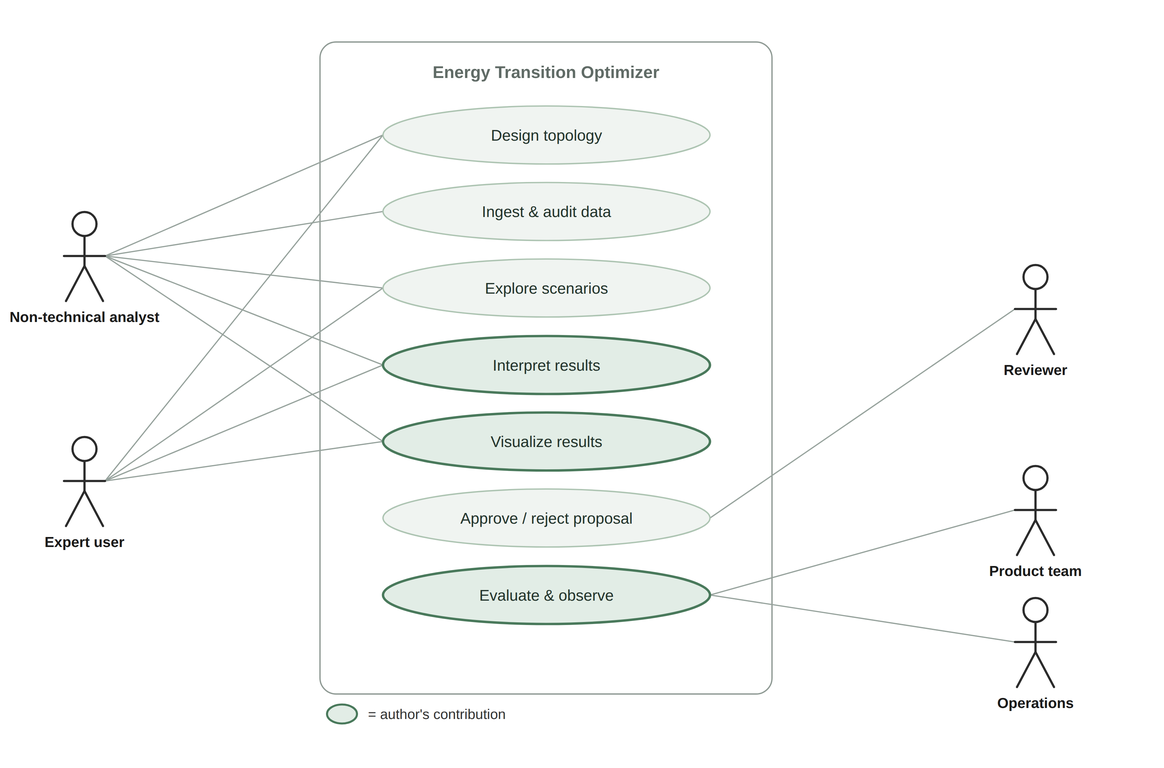
\includegraphics[width=\linewidth]{Figures/usecase.png}
  \caption{Use-case diagram of the governed assistant.}
  \label{fig:usecase}
\end{figure}

\begin{table}[H]
  \centering
  \small
  \begin{tabularx}{\linewidth}{@{}>{\raggedright\arraybackslash}p{3.2cm} >{\raggedright\arraybackslash}X@{}}
    \toprule
    \textbf{Actor} & \textbf{Main use cases} \\
    \midrule
    \textbf{Non-technical analyst} & Design a topology; ingest and audit data;
      explore scenarios; interpret results; visualize results;
      approve or reject proposals. \\
    \addlinespace
    \textbf{Expert user} & All of the above, plus direct use of the deterministic
      product and judgement of proposals. \\
    \addlinespace
    \textbf{Reviewer / approver} & Approve or reject a proposed state change before
      it takes effect. \\
    \addlinespace
    \textbf{BCG~X product team} & Build and maintain the capabilities;
      evaluate assistant behavior; adapt the product for each client. \\
    \addlinespace
    \textbf{Operations and quality} & Observe traces, costs, evaluator scores, and
      platform health. \\
    \bottomrule
  \end{tabularx}
  \caption{Actors and their main use cases.}
  \label{tab:actors}
\end{table}

\section{Functional requirements}
\label{sec:functional}

The functional surface is grouped into capabilities, each stated as a
requirement. These capabilities map onto the stages of a pre-feasibility
study (Figure~\ref{fig:study-workflow}).

\begin{figure}[H]
  \centering
  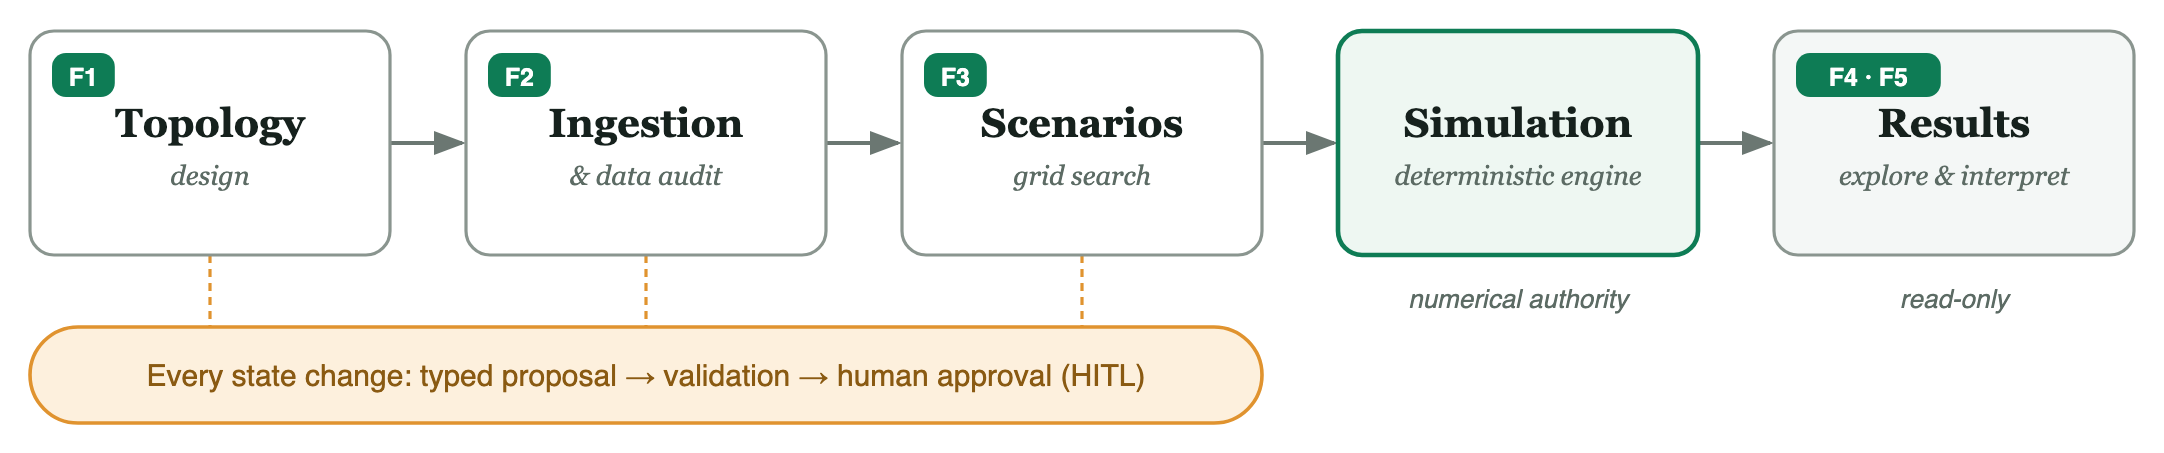
\includegraphics[width=\linewidth]{Figures/study_workflow.png}
  \caption{The end-to-end pre-feasibility study workflow the requirements target,
    with the approval gate on every state-changing stage.}
  \label{fig:study-workflow}
\end{figure}

\begin{description}
  \item[F1. Guided topology design.] From a natural-language description, the
    assistant shall propose a valid project topology (assets, buses, markets, and
    admissible flows), or edit an existing one, and surface the result as a
    reviewable proposal rather than a direct mutation.
  \item[F2. Assumption ingestion and audit.] The assistant shall load uploaded
    assumption files, classify and place their records, detect conflicts with
    existing project data, and return an approval-gated data-quality report.
  \item[F3. Scenario exploration.] The assistant shall help a user turn an intent
    into a bounded set of scenarios (a grid search), proposing sweep values
    across the technical, commercial, financial, and external dimensions, and
    returning a single validated set of operations for approval.
  \item[F4. Result interpretation.] Given a completed simulation
    population, the assistant shall explain, in natural language, which run is
    best, what drives its economics, and which parameters are worth examining,
    with every figure it states traceable to a deterministic result.
  \item[F5. Results visualization.] The interface shall let a user
    explore outputs interactively, including scatter plots with selectable axes
    and a navigable discounted-cash-flow table, and shall offer an
    interpret-on-demand action that attaches a grounded explanation to a chart.
  \item[F6. Governed state changes.] Every state-changing action (topology edit,
    assumption update, scenario submission) shall be expressed as a typed
    proposal, validated against schema and domain rules, and applied only after
    explicit human approval.
  \item[F7. Evaluation of assisted behavior.] The system shall provide
    a means to measure the quality of assistant outputs, scoring the grounding
    and soundness of interpretations and the fidelity of generated structures,
    in a repeatable way across versions.
  \item[F8. Observability and monitoring.] The system shall record traces, model
    usage, and evaluator scores for assisted interactions, and shall support
    periodic health assessment of the deployed platform.
\end{description}

\subsection{Detailed use case: interpreting a completed grid search}

Because result interpretation is central to this work, it is specified as a
detailed scenario.

\begin{description}
  \item[Actor.] Non-technical analyst.
  \item[Precondition.] A grid search has completed and its results are persisted;
    the analyst is viewing the results of a project.
  \item[Main flow.] (1)~The analyst asks, in plain language, to explain a run or
    a chart. (2)~The assistant retrieves the relevant simulation metrics,
    financial breakdowns, and chart context through read-only tools. (3)~It
    produces a streamed narration and a set of insight cards, citing only figures
    read from the deterministic output. (4)~It may embed the relevant chart next
    to the explanation.
  \item[Postcondition.] The analyst obtains a grounded interpretation. No project
    state is modified (the interpreter is read-only), so no approval is required.
  \item[Alternative flow.] If the evidence is insufficient to support a claim
    (for example inferring a correlation from a single point), the assistant
    states the limitation instead of overreaching.
\end{description}

Figure~\ref{fig:interp-usecase} illustrates this scenario on a real study.

\begin{figure}[H]
  \centering
  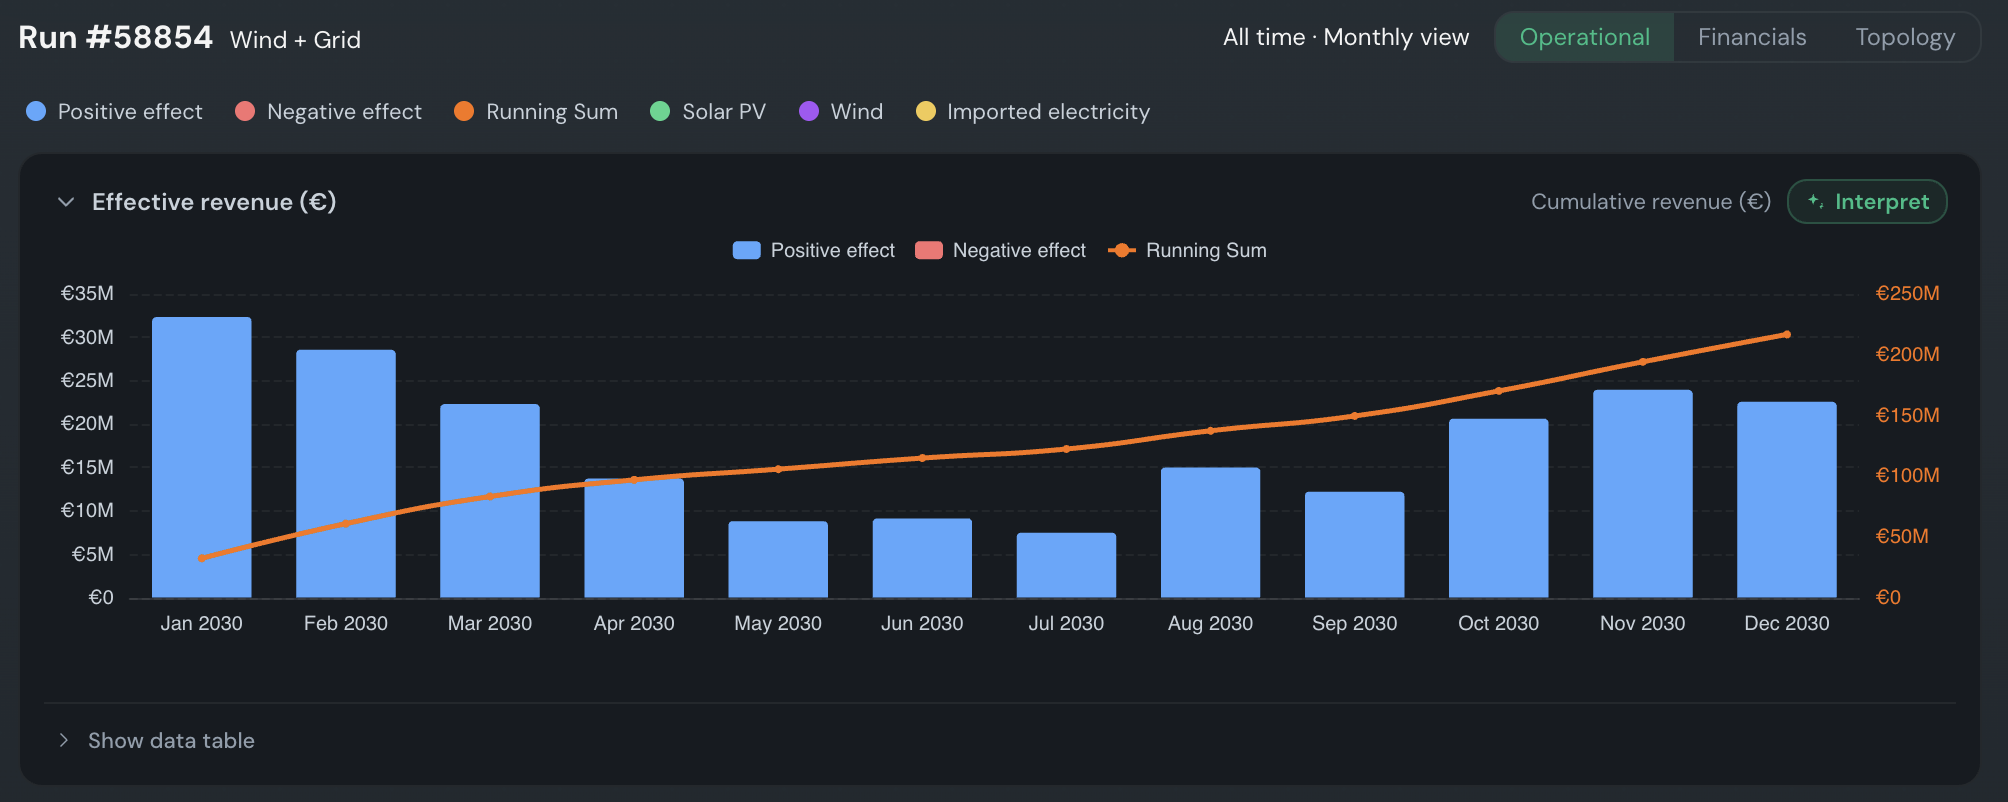
\includegraphics[width=\linewidth]{Figures/1.png}\\[0.3cm]
  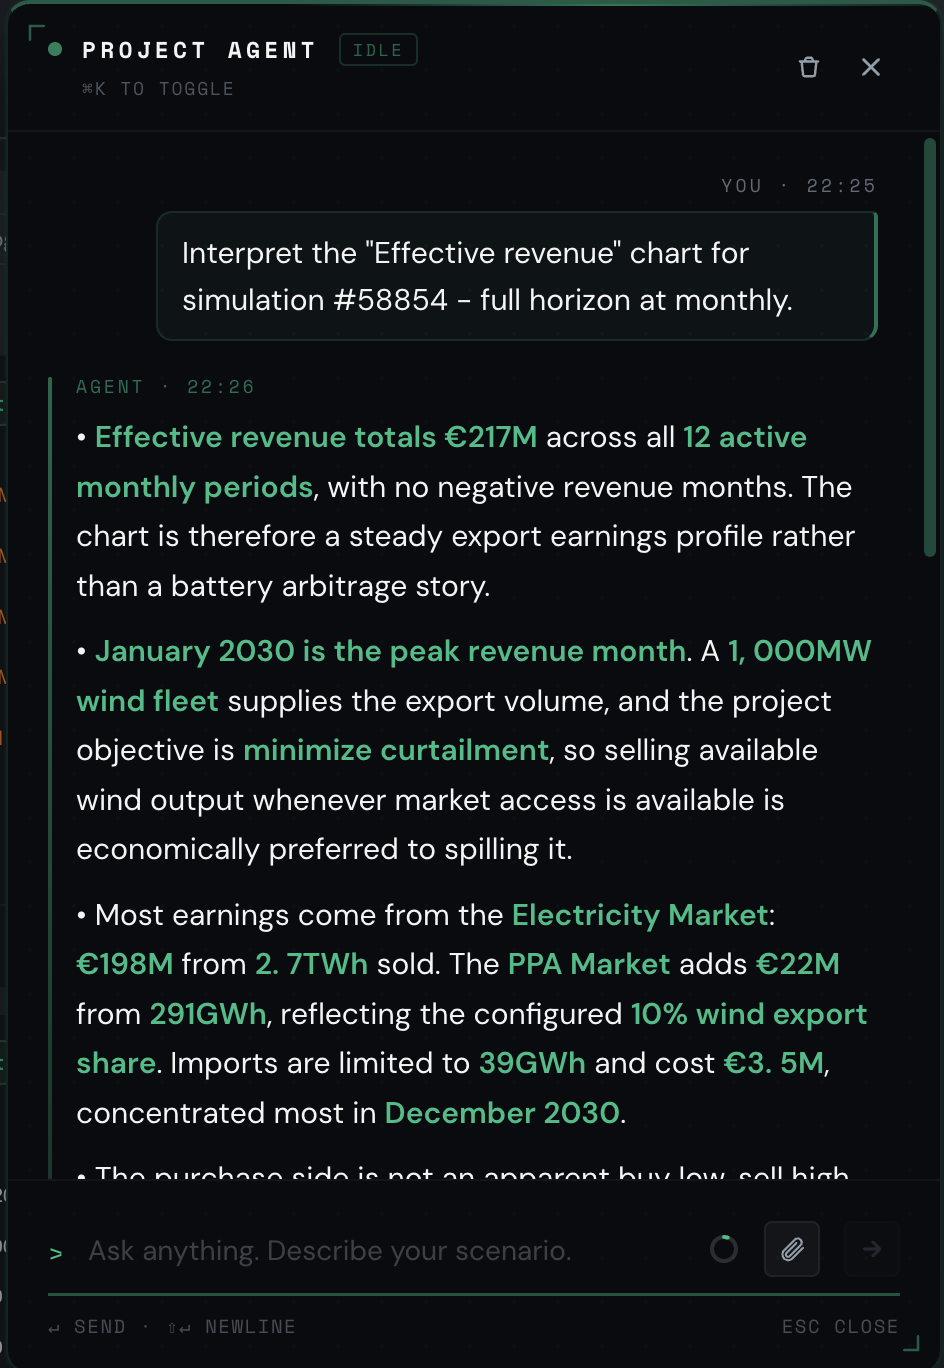
\includegraphics[width=0.32\linewidth]{Figures/2-1.png}
  \hfill
  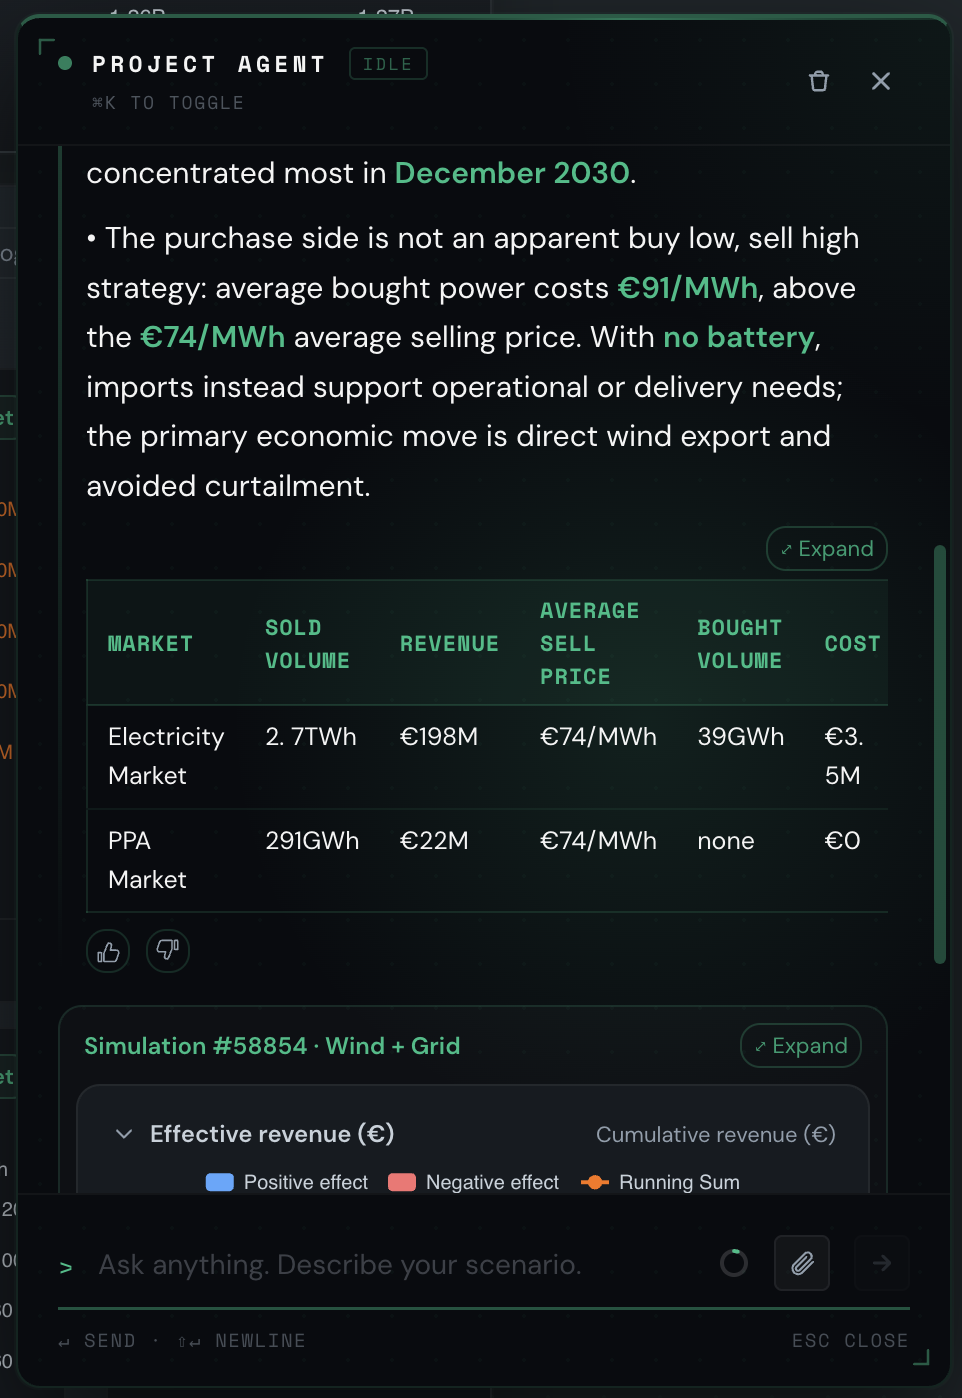
\includegraphics[width=0.32\linewidth]{Figures/2-2.png}
  \hfill
  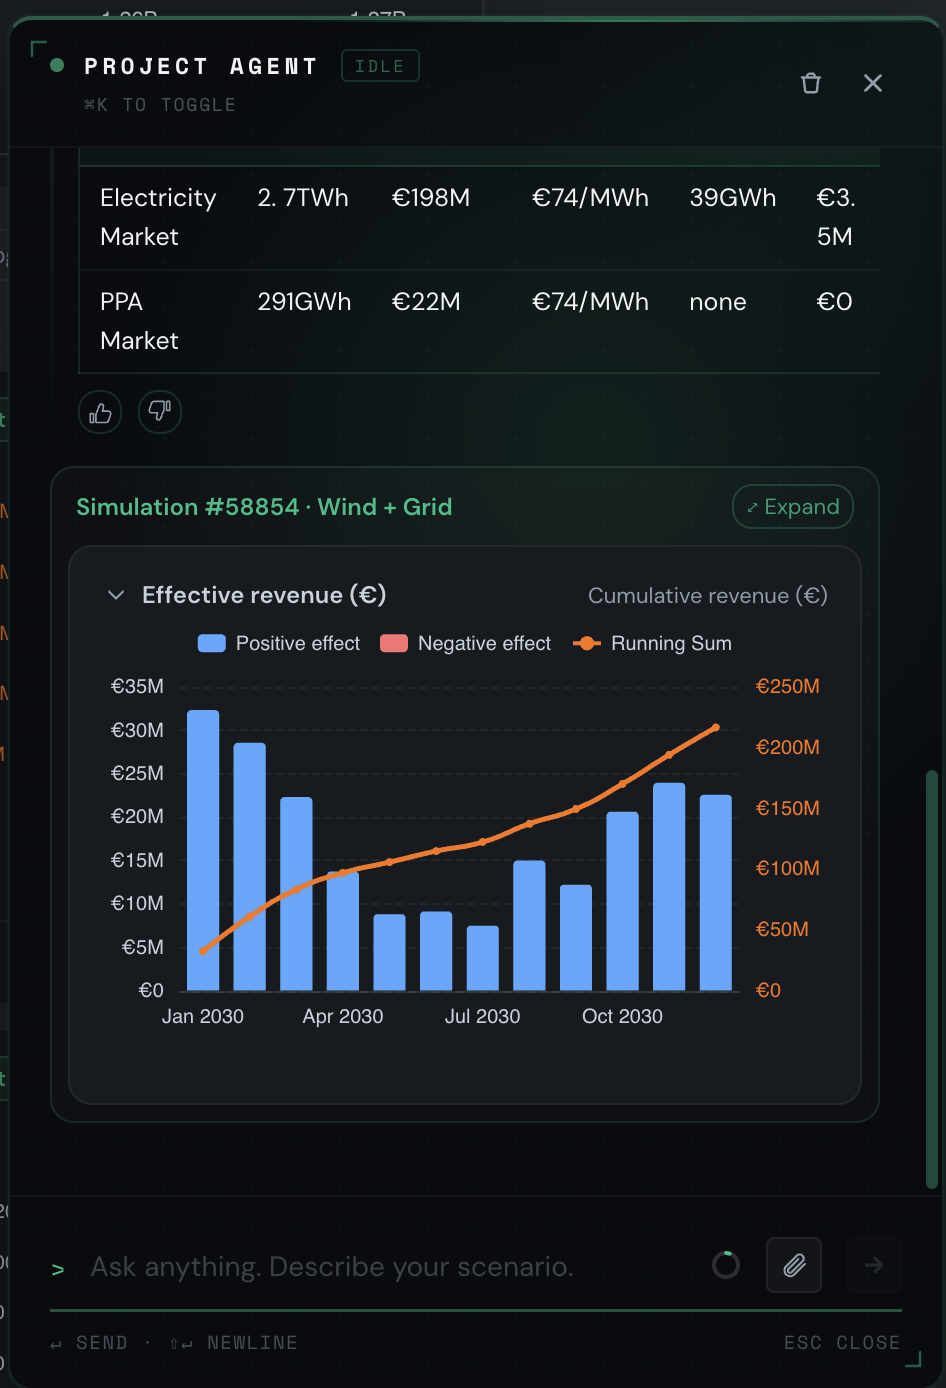
\includegraphics[width=0.32\linewidth]{Figures/2-3.png}
  \caption{The interpreter agent use case.}
  \label{fig:interp-usecase}
\end{figure}

\subsection{Detailed use case: editing a topology under approval}

This second scenario illustrates the governed \emph{write} path, where an action
does change project state and therefore passes through the approval gate.

\begin{description}
  \item[Actor.] Non-technical analyst (with a reviewer, often the same person).
  \item[Precondition.] A project exists; the analyst wants to add or modify an
    asset (for example, ``add a battery and a second electrolyzer'').
  \item[Main flow.] (1)~The analyst describes the change in plain language.
    (2)~The assistant gathers context and generates a candidate topology, then
    validates it against schema and domain rules. (3)~It surfaces the change as a
    \textbf{typed proposal} (a review card), not a direct mutation. (4)~The
    reviewer inspects the proposal and \textbf{approves} it. (5)~Only then is the
    project topology updated. Figure~\ref{fig:topology-design-approval} shows the
    proposal and its approval card.

\begin{figure}[H]
  \centering
  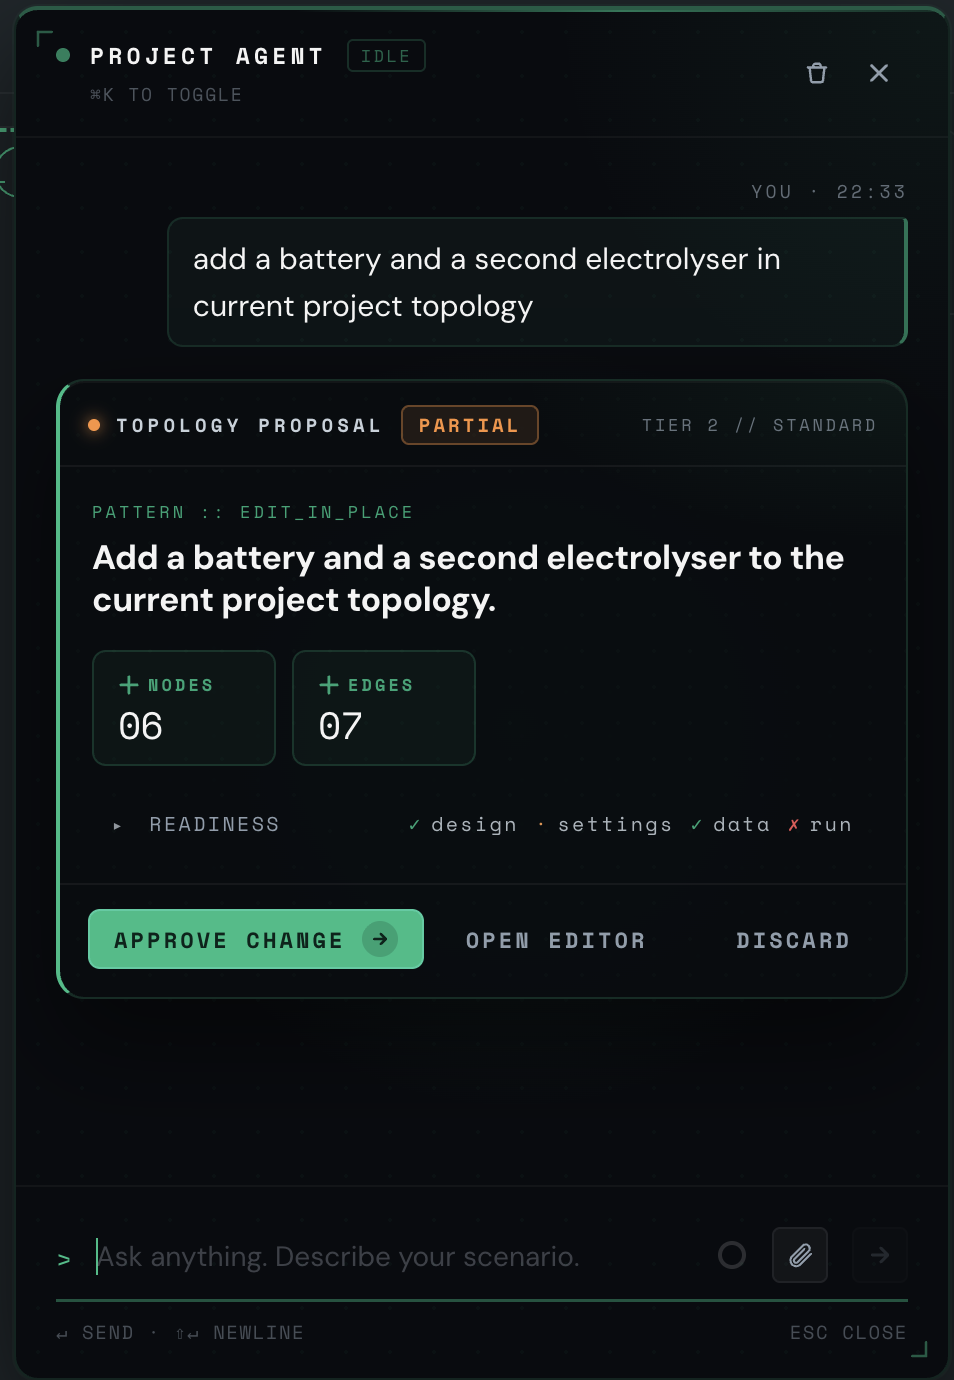
\includegraphics[width=0.48\linewidth]{Figures/a1.png}
  \hfill
  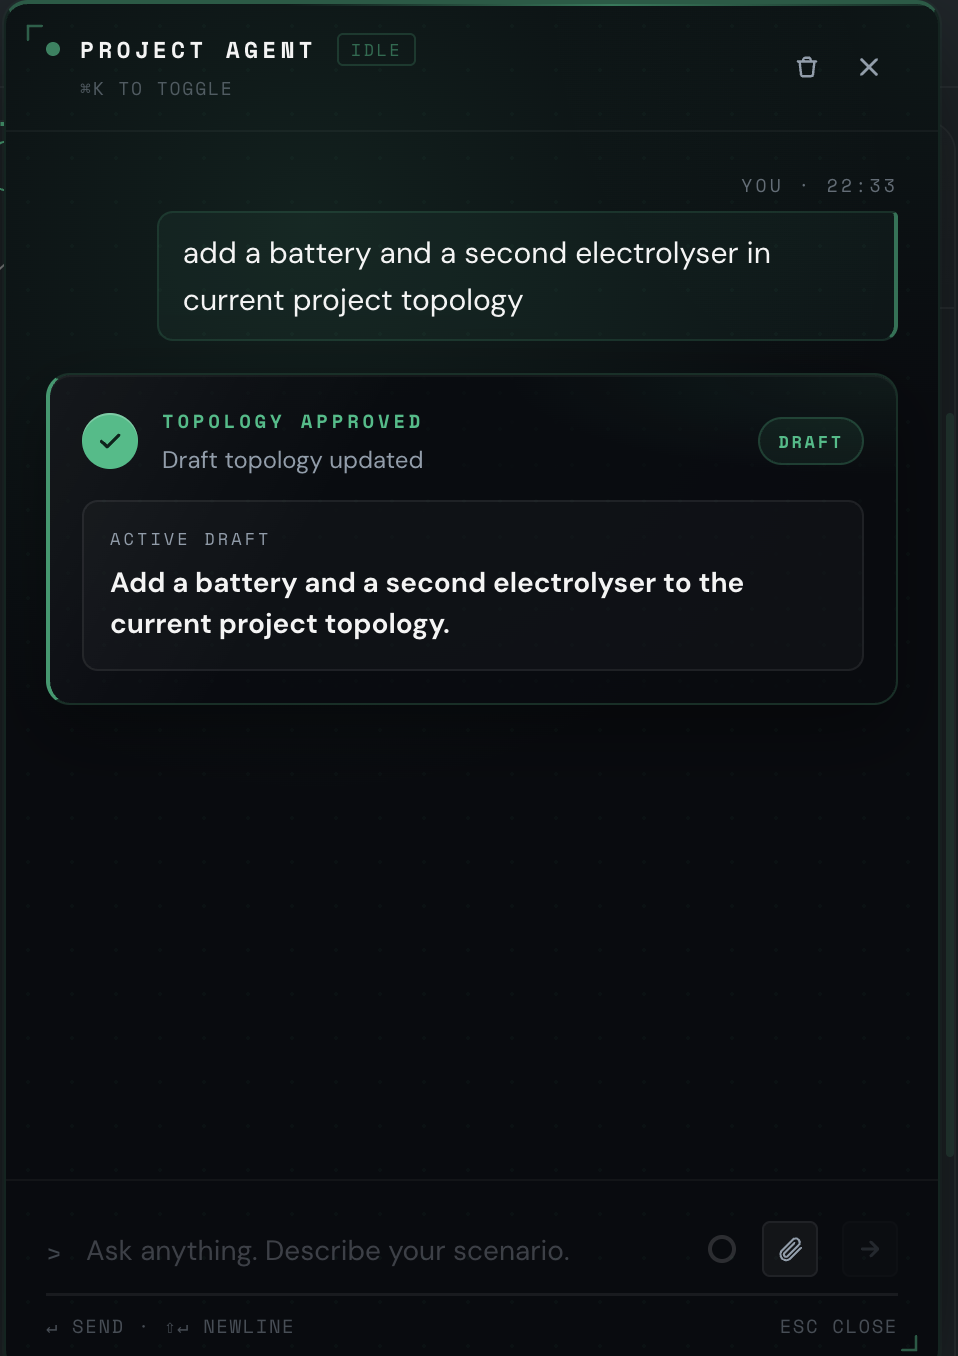
\includegraphics[width=0.48\linewidth]{Figures/a2.png}
  \caption{The topology design use case.}
  \label{fig:topology-design-approval}
\end{figure}

  \item[Postcondition.] The topology is modified in a traceable way, or left
    unchanged if the proposal is rejected.
  \item[Alternative flow.] If validation fails, the assistant blocks the proposal
    and returns the failing evidence rather than applying a broken design; the
    analyst can refine the request and retry.
\end{description}

\section{Non-functional requirements}
\label{sec:nonfunctional}

The non-functional requirements are what make the assistant trustworthy enough to
be used on real analyses; they matter as much as the functional surface.
Table~\ref{tab:nfr} states them with their rationale, and they fall into a few
families. Two express the central principle that the optimizer, not the model, is
the source of truth: \emph{numerical authority} (NF1) and \emph{groundedness}
(NF2), the latter being the property the evaluation harness later measures
directly. Two concern trust in operation, \emph{reproducibility and auditability}
(NF3) and \emph{human control} (NF4), which together make every assisted action
repeatable and reversible under explicit approval. \emph{Responsiveness} (NF5)
keeps the interface usable despite model and simulation latency, and
\emph{evaluability and observability} (NF6) makes agent behavior measurable and
inspectable rather than assumed. Finally, \emph{security and enterprise identity}
(NF7) and \emph{maintainability and adaptability} (NF8) are product-level qualities
that let the same core be operated safely and adapted for each client.

Where useful these carry concrete, testable targets. Interpretations begin
streaming within a short first-token budget rather than blocking on the full
answer (NF5). Structured outputs such as generated topologies are accepted only
above a fixed graph-edit-similarity threshold, set at $0.85$ and tracked across
versions (NF6, Chapter~\ref{chap:implementation}). Interpretations are scored by an
independent judge on groundedness and on financial, commercial, and operational
soundness (NF2, NF6). And every assisted interaction is traced end to end together
with its model usage and evaluator scores (NF6).

\begin{table}[H]
  \centering
  \small
  \begin{tabularx}{\linewidth}{@{}>{\bfseries}l >{\raggedright\arraybackslash}p{3.4cm} >{\raggedright\arraybackslash}X@{}}
    \toprule
    \textbf{Ref.} & \textbf{Requirement} & \textbf{Why it matters} \\
    \midrule
    NF1 & Numerical authority & The deterministic engine remains the sole source
      of results; no figure shown to a user originates from the model. \\
    \hypertarget{nf:groundedness}{NF2} & Groundedness & Every quantitative statement
      is traceable to a specific deterministic output, with no invented numbers. \\
    NF3 & Reproducibility \& auditability & The same inputs give the same results,
      and assisted actions are inspectable after the fact. \\
    NF4 & Human control & No state change takes effect without explicit approval;
      destructive operations are reversible where possible. \\
    NF5 & Responsiveness & Interpretations stream token by token, and long
      computations never block the interface. \\
    \hypertarget{nf:eval}{NF6} & Evaluability \& observability & Behavior is
      measurable through a repeatable harness and observable through end-to-end
      tracing. \\
    NF7 & Security \& enterprise identity & Access is mediated by the enterprise
      identity provider; the application runs no identity stack of its own. \\
    NF8 & Maintainability \& adaptability & Reproducible deployment across the
      several modes, and adaptability to each client. \\
    \bottomrule
  \end{tabularx}
  \caption{Non-functional requirements and their rationale.}
  \label{tab:nfr}
\end{table}

\section{Constraints}
\label{sec:constraints}

Constraints differ from the non-functional requirements above: they are external
givens imposed on the work rather than quality targets it sets for itself. Several
are \emph{realized} by a non-functional requirement, noted below so the two are not
read as duplicates.

\begin{itemize}
  \item \textbf{Deterministic authority.} The founding premise of the project: the
    assistant assists and proposes but never computes final results. It is imposed
    here, and the design turns it into numerical authority (NF1) and human control
    (NF4).
  \item \textbf{Client confidentiality.} No client-identifying data appears in the
    product artifacts or in this report; the product is an internal asset adapted
    per client (Section~\ref{sec:internal-product}). This is a business and legal
    given, with no functional substitute.
  \item \textbf{Enterprise identity.} The host organization mandates that
    authentication be delegated to its own identity provider through OpenID
    Connect; the design meets this through NF7.
  \item \textbf{Model cost and latency.} Language-model calls carry a cost and a
    latency budget the work does not control; the design respects it (for example
    by reusing prior results and streaming output), the user-facing side of which
    is NF5.
\end{itemize}

Reproducibility across the local, container, and cloud modes is likewise required,
but as a quality target it is stated as a non-functional requirement (NF8) rather
than repeated here.

\section{Prioritization}
\label{sec:prioritization}

The functional requirements were prioritized using a MoSCoW scheme. Within the
scope of this report every functional requirement is either a \emph{Must} or a
\emph{Should}; none were deferred to \emph{Could} or \emph{Won't}, so those tiers
do not appear. The priorities reflect this phase of the work rather than a
from-scratch build order. Governed state changes
(F6) is \emph{Must} because it is the safety foundation every other capability
depends on: it is the condition under
which any assisted capability may touch project state. Result interpretation
(F4), visualization (F5), and evaluation (F7) are \emph{Must} because they close
the loop the project set out to deliver: results that can be explored, explained,
and trusted. Guided topology design (F1), ingestion (F2), scenario exploration
(F3), and observability (F8) are logically prior to interpretation in a study but
were largely already in place when this phase of the work began, so they are
\emph{Should}. The non-functional
requirements are treated as qualities that must hold throughout rather than ranked
on the same scale. Table~\ref{tab:prio} summarizes the result.

\begin{table}[H]
  \centering
  \small
  \begin{tabularx}{\linewidth}{@{}>{\bfseries}l >{\raggedright\arraybackslash}X >{\centering\arraybackslash}p{2.4cm}@{}}
    \toprule
    \textbf{Ref.} & \textbf{Requirement} & \textbf{Priority} \\
    \midrule
    F6 & Governed state changes & Must \\
    F4 & Result interpretation & Must \\
    F5 & Results visualization & Must \\
    F7 & Evaluation of behavior & Must \\
    F1 & Guided topology design & Should \\
    F2 & Assumption ingestion and audit & Should \\
    F3 & Scenario exploration & Should \\
    F8 & Observability and monitoring & Should \\
    \bottomrule
  \end{tabularx}
  \caption{Prioritization of functional requirements.}
  \label{tab:prio}
\end{table}

\section*{Conclusion}

This chapter specified the actors, the functional requirements grouped by
capability, the non-functional requirements that establish trust, the binding
constraints, and the prioritization of the work, with result interpretation,
visualization, evaluation, and governed state changes identified as the
capabilities the project had to deliver end to end. The next chapter presents
the design and architecture that satisfy these requirements.
